\documentclass[12pt]{report}
\usepackage[a4paper]{geometry}
\usepackage[utf8]{inputenc}
\usepackage[english,portuguese]{babel}
\usepackage[myheadings]{fullpage}
\usepackage[T1]{fontenc}
\usepackage{fancyhdr}
\usepackage{graphicx, setspace}
\usepackage{sectsty}
\usepackage{url}
\usepackage{pdfpages}
\usepackage{subcaption}
\usepackage{amsmath}
\usepackage{multirow}
\usepackage{tikz}
\usepackage{minted}
\usepackage{hyperref}
\usepackage{amsfonts}
\usepackage{mathtools, amsmath}

%%------ 
%% Comandos gerais
%% Observação: o arquivo "comandos.tex" tem que estar presente.
%%------
%%%%%%%%%%%%%%%%%%%%%%%%%%%%%%%%%%%%%%%%%%%%%%%%%%%%%%%%%%%%%%%%%%%%%
% In English:
%    This is a list of commands specification for FAPESP reports.
%
% In Portuguese:
%    Esta é uma lista de especificação de comandos para relatórios
% da Fundação de Amparo à pesquisa do Estado de São Paulo (FAPESP).
%
% Author/Autor: André Leon Sampaio Gradvohl, Dr.
% Email:        andre.gradvohl@gmail.com
% Lattes CV:    http://lattes.cnpq.br/9343261628675642
% 
% Last update/Última versão: 11/Sep/2016
%%%%%%%%%%%%%%%%%%%%%%%%%%%%%%%%%%%%%%%%%%%%%%%%%%%%%%%%%%%%%%%%%%%%%%

\def\checkmark{\tikz\fill[scale=0.4](0,.35) -- (.25,0) -- (1,.7) -- (.25,.15) -- cycle;}

\DeclareMathOperator{\diag}{diag}
\DeclareMathOperator{\ai}{Ai}
\DeclareMathOperator{\re}{Re}
\DeclareMathOperator{\im}{Im}
\DeclareMathOperator{\ee}{\rm e}
\DeclareMathOperator{\supp}{supp}
\renewcommand{\Re}{\mathop{\rm Re}}
\newcommand{\res}{\mathop{\rm Res}}
\renewcommand{\Im}{\mathop{\rm Im}}
\newcommand{\N}{\mathbb{N}}
\newcommand{\C}{\mathbb{C}}
\DeclareMathOperator{\Tr}{Tr}
\newcommand{\R}{\mathbb{R}}
\newcommand{\Z}{\mathbb{Z}}
\newcommand{\D}{\mathbb{D}}
\newcommand{\Q}{\mathbb{Q}}
\newcommand{\boh}{\mathit{o}}
\newcommand{\Boh}{\mathcal{O}}
\newcommand{\bbp}{\bm K_{\mathrm{BBP}}}
\newcommand{\ii}{\mathrm{i}}
\newcommand{\dd}{\mathrm{d}}
\newcommand*{\deff}{\mathrel{\vcenter{\baselineskip0.5ex \lineskiplimit0pt
			\hbox{\scriptsize.}\hbox{\scriptsize.}}}%
	=}
\newcommand*{\revdeff}{=\mathrel{\vcenter{\baselineskip0.5ex \lineskiplimit0pt
			\hbox{\scriptsize.}\hbox{\scriptsize.}}}%
}

\newcommand{\HRule}[1]{\rule{\linewidth}{#1}}
\setcounter{tocdepth}{3}
\setcounter{secnumdepth}{3}

\newcommand{\titulo}[1]{\def\meuTitulo{#1}}
\newcommand{\tituloIngles}[1]{\def\meuTituloIngles{#1}}
\newcommand{\numProjeto}[1]{\def\numFAP{#1}}
\newcommand{\tipoRelatorio}[1]{\def\tipoRelat{#1 }} %o espaço depois do #1 é importante
\newcommand{\modalidadeProjeto}[1]{\def\modProjeto{#1}} 
\newcommand{\agFomento}[2]{\def\agFom{#1} \def\siglaAgFom{#2}} %extenso Sigla
\newcommand{\autor}[1]{\def\nomeAutor{#1}}
\newcommand{\cidade}[1]{\def\nomeCidade{#1}}
\newcommand{\universidade}[1]{\def\nomeUniversidade{#1}}
\newcommand{\faculdade}[1]{\def\nomeFaculdade{#1}}
\newcommand{\periodoVigencia}[1]{\def\periodVig{#1}}
\newcommand{\periodoRelatorio}[1]{\def\periodRelat{#1}}

\author{}
\date{}

%Definição de membros da equipe de pesquisas
\newcommand{\membroA}[1]{\def\nomeMembroA{#1}}
\newcommand{\membroB}[1]{\def\nomeMembroB{#1}}
\newcommand{\membroC}[1]{\def\nomeMembroC{#1}}
\newcommand{\membroD}[1]{\def\nomeMembroD{#1}}
\newcommand{\membroE}[1]{\def\nomeMembroE{#1}}
\newcommand{\membroF}[1]{\def\nomeMembroF{#1}}

\newcommand{\Figure}[1]{Figura~\ref{fig:#1}}
\newcommand{\Table}[1] {Tabela~\ref{#1}}
\newcommand{\Equation}[1] {Equa\c{c}\~ao~\ref{#1}}
\newcommand{\addFigure}[3] { %Parametros scale, fig_name, caption 
    \begin{figure}[!hbt]
      \centering
      \includegraphics[scale=#1]{figures/}
      \caption{#3}\label{fig:#2}
    \end{figure}
}

\newcommand{\geraTitulo}{
\clearpage
\begin{titlepage}
  \begin{center}
      \vspace*{-3cm}
       { \setstretch{.5} 
         \textsc{\nomeUniversidade} \\
         \HRule{.2pt}\\
         \textsc{\nomeFaculdade}
       }

       \vspace{5.5cm}

       \Large \textbf{\textsc{\meuTitulo}}
 	  \HRule{1.5pt} \\ [0.5cm]
       \linespread{1}
       \large Relatório Científico 
       \ifdefined\tipoRelat
            \tipoRelat
       \fi
       do projeto 
       \ifdefined\modProjeto
           na modalidade \modProjeto,
       \fi
       fomentado pela \agFom. \\ 
   	   \HRule{1.5pt} \\ [0.5cm]

       \ifdefined\numFAP
          Projeto \siglaAgFom~\texttt{\#\numFAP}
          \\ [0.5cm]
       \fi
        Pesquisador Responsável: \nomeAutor
        
        \hspace{2cm}
        
        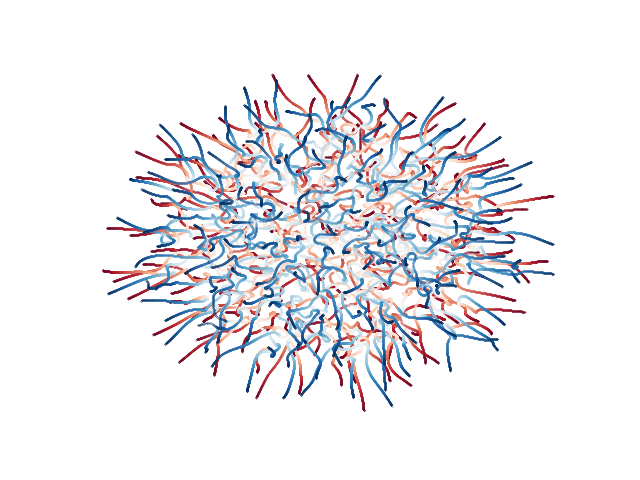
\includegraphics[scale=0.7]{Assets/CuteCircleWhite}
       
        \vfill
       
        {\normalsize  \nomeCidade, \today}
 \end{center}
 \end{titlepage}
}

\usepackage{titlesec}
\titleformat{\chapter}{\normalfont\LARGE\bfseries}{\thechapter}{1em}{}
\titlespacing*{\chapter}{0pt}{3.5ex plus 1ex minus .2ex}{2.3ex plus .2ex}

%----------------------------------------------------------------------
% Cabeçalho e rodapé
%----------------------------------------------------------------------
\pagestyle{fancy}
\fancyhf{} % Limpa todos os campos de header and footer fields
\renewcommand{\headrulewidth}{0pt}
\fancyfoot[R]{\thepage}

\addto\captionsportuguese{\renewcommand{\contentsname}{Sumário}}
\addto\captionsportuguese{\renewcommand{\bibname}{Referências Bibliográficas}}

%------
% Resumo e Abstract
%------
\newcommand{\Resumo}[1]{
   \begin{otherlanguage}{portuguese}
       \addcontentsline{toc}{chapter}{Resumo}
       \begin{abstract} \thispagestyle{plain} \setcounter{page}{2}
          #1
        \end{abstract}
   \end{otherlanguage} 
} %end \Resumo

\newcommand{\Abstract}[1]{
   \begin{otherlanguage}{english}
      \addcontentsline{toc}{chapter}{Abstract}
      \begin{abstract} \thispagestyle{plain} \setcounter{page}{3}
       #1
      \end{abstract}    
    \end{otherlanguage} 
} %end \abstract

%------
% Folha de rosto
%------
\newcommand{\folhaDeRosto}{
   \chapter*{Informações Gerais do Projeto}
   \addcontentsline{toc}{chapter}{Informações Gerais do Projeto}
   \begin{itemize}
      \item Título do projeto: 
            \begin{itemize}\item[] \textbf{\meuTitulo} \end{itemize}
      \item Nome do pesquisador responsável: 
            \begin{itemize}\item[]\textbf{\nomeAutor}\end{itemize}
      \item Instituição sede do projeto: 
            \begin{itemize}
               \item[]\textbf{\nomeFaculdade \ da \nomeUniversidade} 
            \end{itemize}
      \item Equipe de pesquisa:
            \begin{itemize}
               \ifdefined\nomeMembroA
                 \item[]\textbf{\nomeMembroA}
               \else 
                 \item[]\textbf{\nomeAutor}
               \fi
               \ifx\nomeMembroB\undefined\else \item[]\textbf{\nomeMembroB}\fi
               \ifx\nomeMembroC\undefined\else \item[]\textbf{\nomeMembroC}\fi
               \ifx\nomeMembroD\undefined\else \item[]\textbf{\nomeMembroD}\fi
               \ifx\nomeMembroE\undefined\else \item[]\textbf{\nomeMembroE}\fi
               \ifx\nomeMembroF\undefined\else \item[]\textbf{\nomeMembroF}\fi
             \end{itemize}
       
          \ifdefined \numFAP
             \item Número do projeto de pesquisa:
             \begin{itemize}
                 \item[]\textbf{\numFAP} 
             \end{itemize}
          \fi  
       \item Período de vigência:
            \begin{itemize}
               \item[]\textbf{\periodRelat} 
            \end{itemize}
       \item Período coberto por este relatório científico:
            \begin{itemize}
               \item[]\textbf{\periodVig} 
            \end{itemize}
   \end{itemize}
   \clearpage
}


\newcommand\underrel[2]{\mathrel{\mathop{#2}\limits_{#1}}}

\newcommand{\matriz}[1]{\hat#1}

\newcommand{\many}[2]{$#1_1, #1_2, \dots, #1_#2$}

\newcommand{\cmany}[3]{$#1_1 #3 #1_2 #3 \dots #3 #1_#2$}

\newcommand{\mmany}[2]{ #1_1, #1_2, \dots, #1_#2 }

\newcommand{\mcmany}[3]{#1_1 #3 #1_2 #3 \dots #3 #1_#2}

\newcommand{\set}[1]{\{#1\}}

\newcommand{\cjgt}[1]{\overline{#1}}
\DeclareMathOperator{\sign}{sign}
\DeclareMathOperator{\Df}{D}
\DeclareMathOperator{\Ee}{E}
\DeclareMathOperator{\h}{h_1}
\DeclareMathOperator{\f}{f}
\DeclareMathOperator{\U}{U}
\DeclareMathOperator{\W}{W}
\DeclareMathOperator{\K}{K}
\DeclareMathOperator{\Hf}{\mathcal{H}}
\DeclareMathOperator{\Qf}{Q}
\DeclareMathOperator{\Gl}{\mathcal{L}}
\DeclareMathOperator{\g}{g}
\DeclareMathOperator{\V}{V}
\newcommand{\iu}{\mathrm{i}\mkern1mu}
\renewcommand{\Im}{\mathop{\textrm Im}}
\newcommand{\J}{J} %Jacobiano
\newcommand{\Id}{\mathbb{1}}
\newcommand{\p}{\mathcal{P}} %medida
\newcommand{\Se}{\mathbb{S}}
\newcommand{\He}{\mathbb{H}}
 \newcommand{\E}{\mathbb{E}}

% MATH DECLARATIONS
\newtheorem{lemma}{Lema}[section]
\newtheorem{thm}[lemma]{Teorema}
\newtheorem{claim}[lemma]{Afirmação}
\newtheorem{cor}[lemma]{Corolário}
\newtheorem{definition}[lemma]{Definição}
\newtheorem{conjecture}[lemma]{Conjectura}
\newtheorem{prop}[lemma]{Proposição}
\newtheorem{assumption}[lemma]{Assumpção}
\numberwithin{equation}{section} %numeracao dentro de secoes

% PROOF ENV
\makeatletter
\newenvironment{proof}[1][Demonstração]{\par
	\pushQED{\qed}%
	\normalfont \topsep6\p@\@plus6\p@\relax
	\trivlist
	\item\relax
	{\itshape
		#1\@addpunct{.}}\hspace\labelsep\ignorespaces
}{%
	\popQED\endtrivlist\@endpefalse
}
\makeatother
%
%%-----
%% Página de título
%% Observação: As definições que aparecem a seguir comporão a
%%             página de título e a folha de rosto.
%%-----
%% Define o nome da universidade onde o projeto foi desenvolvido.
\universidade{Universidade de São Paulo}
%
%% Define o nome da faculdade onde o projeto foi desenvolvido.
\faculdade{Instituto de Ciências Matemáticas e de Computação (ICMC)}
%
%% Define o título do projeto.
\titulo{Matrizes aleatórias e simulação de gases de Coulomb}
%
%% Define a agencia de Fomento e a abreviatura. O primeiro argumento é o 
%% nome por extenso e o segundo a abreviatura.
%% Ambos os argumentos são obrigatórios
\agFomento{Fundação de Amparo à Pesquisa do Estado de São Paulo}{FAPESP}
%
%% Define o tipo de relatório. Pode ser Anual ou Final.
%% Não é obrigatório definir o tipo de relatório.
\tipoRelatorio{semestral}
%
%% Define a modalidade de Projeto. Pode ser temático, regular, etc.
\modalidadeProjeto{iniciação científica}
%
%% Define o número do projeto.
%% Não é obrigatório definir o número do projeto.
\numProjeto{2023/02674-0} 
%
%% Define o autor do relatório.
\autor{Guilherme L. F. Silva}
%
%% Define a equipe do projeto (incluindo o pesquisador responsável no comando \membroA{}
\membroA{Guilherme L. F. Silva}
%% Inclua os demais membros do grupo (máximo +5)
\membroB{João Victor Alcantara Pimenta}
%\membroC{Francisco}
%\membroD{Joao}
%\membroE{Antonio}
%\membroF{José}
%
%% Define o período da vigência do Projeto.
\periodoVigencia{01/06/2023 a 31/05/2024}
%
%% Define o período coberto pelo relatório.
\periodoRelatorio{01/06/2023 a 10/11/2023}
%
%% Define a cidade onde o projeto foi desenvolvido.
\cidade{São Carlos}

%%-----
%% Página de título
%% Observação: Os comandos a seguir não devem ser mudados, 
%%             exceto caso necessário.
%%-----
\begin{document}
	%
	%% Define a numeração em romanos.
	\pagenumbering{roman}
	%
	%% Gera a folha de título.
	\geraTitulo
	%
	%% Gera a folha de rosto.
	\folhaDeRosto
	%
	%% Escreva aqui o resumo em português.
	\Resumo{O estudo de Matrizes Aleatórias demonstra aplicabilidade em uma gama diversa de áreas, com destaque no estudo de mecânica estatística, principalmente na simulação de gases. Estudando a densidade espectral de sistemas de matrizes Gaussianas pode-se desenvolver uma analogia que possibilita a simulação de sistemas de gases diversos, como o de Coulomb. Algumas dificuldades surgem na implementação de simulações baseadas nesta teoria, principalmente em escalabilidade do sistema e no tratamento de possíveis singularidades. Para resolver estes problemas, abordou-se na simulação na literatura, dentre outros, o Algoritmo Híbrido de Monte Carlo, de ótimo comportamento numérico. Nosso objetivo é explorar este assunto, as simulações de gases e o algoritmo citado acima além de expandir os potenciais em que foi-se bem documentado o comportamento destas simulações.}
	%
	%% Escreva aqui o resumo em inglês.
	% \Abstract{
		%	The study of Random Matrices demonstrates applicability in a diverse range of areas, empha-
		%	sizing the study of statistical mechanics, mainly in the simulation of gases. By studying the
		%	spectral density of Gaussian matrix systems, one can develop the simulation of Coulomb gas
		%	systems in analogy. Some difficulties arise in implementing simulations based on this theory,
		%	mainly in system scalability and the treatment of possible singularities. To solve these pro-
		%	blems, the literature has simulated these gases, with excellent numerical behavior, using the
		%	Monte Carlo Hybrid Algorithm. We wish to explore this problem, the simulations, and the
		%	proposed algorithm along with extending the potentials to wich it has been tested.
		%}
	%
	%% Adicionará o sumário.
	%% Mantenha o \thispagestyle{empty} e \clearpage
	\thispagestyle{empty}
	\clearpage
	%
	%% Define a numeração em arábicos.
	\pagenumbering{arabic}
	
	%%-----
	%% Formatação do título da seção
	%%-----
	\sectionfont{\scshape}
	
	%%-----
	%% Corpo do texto
	%%-----
	
	{\let\clearpage\relax \chapter{Realizações do período}}
	\label{chp:realizacoes}
	
	\section{Graduação}
	
	Durante o período referente ao relatório o aluno completou as matérias do primeiro semestre e iniciou as matérias do segundo semestre listadas na tabela abaixo.
	
	\hspace{1cm}
	
	\begin{center}
		\begin{tabular}{|c|c|c|c|}
			\hline
			Disciplina & Sigla & Nota & Semestre \\
			\hline
			Mecânica Estatística Avançada & 7600041 & 10.0 & 1 - 2023 \\
			\hline
			Introdução aos Sistemas de Computação & 7600056 & 9.2 & 1 - 2023 \\
			\hline
			Física Estatística Computacional & 7600073 & 9.7 & 1 - 2023 \\
			\hline
			Teoria Espectral de Matrizes & SME0243 & 10.0 & 1 - 2023 \\
			\hline
			Mecânica Quântica & 7600022 & - & 2 - 2023 \\
			\hline
			Física Matemática Avançada & 7600034 & - & 2 - 2023 \\
			\hline
			Noções Básicas de Fabricação Mecânica & 7600134 & - & 2 - 2023 \\
			\hline
			Espaços Métricos & SMA0343 & - & 2 - 2023 \\
			\hline
			Trabalho de Conclusão de Curso & 7600039 & - & 2 - 2023 \\
			\hline
		\end{tabular}
	\end{center}
	
	\section{Produções}
	
	No período referido foi também submetido na plataforma do Arxiv o pre-print do artigo do qual sou co-autor. O arquivo pode ser encontrado em \href{https://doi.org/10.48550/arXiv.2310.17083}{A Central Theorem for intransitive dice} (https://doi.org/10.48550/arXiv.2310.17083).
	
	\section{Pesquisa}
	
	Durante os meses referentes a esse relatório grande parte do esforço foi no estudo da bibliografia e conteúdo de interesse dentro da teoria de matrizes aleatórias. Para isso, permitiu-se exploração ampla de conceitos relacionados e implementação de algoritmos especiais em interesse ao aluno. Alguns dos principais projetos foram nos temas
	
	\begin{itemize}
		\item Simulação da distribuição de ensembles clássicos de matrizes aleatórias a serem explicitados no relatório (GUE, GOE, GSE);
		\item Movimentos brownianos não interseccionantes e variações de interesse com múltiplos pontos finais da dinâmica;
		\item Métodos de \textit{tilings} baseados em teoria de matrizes aleatórias, tais como o círculo ártico;
		\item Processos de borda das dinâmicas anteriormente citadas e explicitação de distribuições como a Tracy Widow;
	\end{itemize}
	
	Todos os resultados computacionais e implementações realizadas podem ser encontrados em \href{https://github.com/Joao-vap/RMT-Code/tree/main}{GitHub - Repositório Geral} (https://github.com/Joao-vap/RMT-Code/tree/main). 
	
	A outra principal atividade realizada foi a implementação do algoritmo descrito na referência \cite{Chafa__2018}, onde podemos simular algumas medidas de probabilidade relacionadas à ensembles clássicos para validar seu funcionamento. Como é possível ver em \ref{fig: semicircle}, simulamos a distribuição para a GOE, GUE e GSE. Podemos ver nas imagens a concordância das simulações com o método clássico utilizando autovalores de ensembles de matrizes aleatórias. Estendemos também os resultados para alguns potenciais de medida conhecida, mônico e quártico, ainda em validação numérica. 
	
	\section{Introdução à Matrizes Aleatórias}\label{chp:resumoProj} 
	
	Uma matriz aleatória é uma matriz cujas entradas são variáveis aleatórias, não necessariamente independentes tampouco de mesma distribuição. A princípio, de um ponto de vista puramente analítico, pode-se tratar uma matriz aleatória de tamanho $N\times N$ como um vetor aleatório de tamanho $N^2$. No entanto, as estruturas algébrico-geométricas presentes a matrizes, como multiplicação natural, interpretação como operadores, ou decomposições espectrais, trazem à matrizes aleatórias aplicações múltiplas. Em particular, sua relevância estende um ponto comum que compartilham com variáveis aleatórias: permitir descrições estatísticas a sistemas e fenômenos. 
	
	É comum modelar com matrizes aleatórias, por exemplo, operadores com perturbações aleatórias. De um ponto de vista físico, autovalores de um dado operador descrevem espectros de energia do sistema descrito. Na quântica, por exemplo, autovalores são as medidas observadas. Surge uma pergunta naturalmente: dada uma matriz aleatória $M$, o que podemos dizer sobre estatísticas de seus autovalores? Essa resposta, claro, depende de maneira altamente não trivial das distribuições das entradas.  
	
	\section{Distribuição dos Autovalores}
	
	Consideraremos no nosso estudo para referencia matrizes quadradas de entradas complexas com dimensão $N$. Nosso objetivo é afinal ter uma forma de mensurar a distribuição de autovalores e para isso, faremos os seguintes desenvolvimentos.

Consideremos inicialmente um espaço de matrizes com entradas complexas $2N^2$ dimensional. Contido neste espaço temos um espaço de maior interesse correspondente ao espaço das matrizes \textit{hermitianas} de dimensão $N^2$. A escolha do subespaço está relacionada com o fato que matrizes hermitianas são diagonalizáveis e a distribuição de seus autovalores estará diretamente relacionada (com uma mudança de base) à distribuição do traço da matriz diagonalizada. Note que para a matriz diagonal ter a mesma medida que nossa matriz inicial, nossa medida deve ser invariável por rotação.

Mais detalhadamente podemos escrever nossa matriz hermitiana $\matriz{H}$ como 

\[
\matriz{H} = \matriz{U} \matriz{\Lambda} \matriz{U}^{-1} \ , \ \matriz{\Lambda} = diag(\lambda_1, \dots, \lambda_2) \ , \ \matriz{U}\cdot\matriz{U}^* = I
\]

onde, claro, $\matriz{\Lambda}$ é diagonal de autovalores e $\matriz{U}$ é unitária e com colunas equivalentes aos autovetores de $\matriz{H}$. Em geral, o conjunto de matrizes degeneradas tem medida nula e não é uma preocupação. Um cuidado deve ser tomado. A correspondência $\matriz{H} \implies (\matriz{U} \ U(N), \matriz{\Lambda})$ não é injetora, podemos tomar $\matriz{U}_1 \matriz{\Lambda} \matriz{U}_1^{-1} = \matriz{U}_2 \matriz{\Lambda} \matriz{U}_2^{-1}$ se $\matriz{U}_1^{-1} \matriz{U}_2 = diag(e^i\phi_1, \dots, e^i\phi_N)$ para qualquer escolha de fases $(\phi_1, \dots, \phi_N)$. Para restringir nosso problema e tornar a função injetiva será necessário considerar as matrizes unitárias ao espaço de coset $U(N) / U(1) \times \dots \times U(1)$ \footnote{Não tenho muita ideia de espaços de Coset. Pelo que entendo, existe um espaço onde toda $\matriz{U}$ pode ser representada por $\matriz{U}_c \matriz{U}_d$, onde $\matriz{U}_c$ compõe o espaço de coset e $\matriz{U}_d$ é uma matriz diagonal unitária. Dessa forma matrizes equivalentes são aquelas que multiplicadas por $\matriz{U}_d$ tem um mesmo resultado.}. Uma outra restrição necessárias é ordenas os autovalores, ou seja, $\lambda_1 < \dots < \lambda_n$. Temos que reescrever agora a medida $d\mu(\matriz{H})$ em função de auvalores e da $\matriz{U}$ de autovetores.

Para resumir o desenvolvimento, alguns resultados serão diretamente enunciados. Essa seção pode ser encontrada no relatório \cite{fyodorov2010introduction}. Em especial recuperaremos o elemento de distância e volume no subespaço que vamos tratar

\begin{equation}
	(ds)^2 = \Tr{d\matriz{H} d\matriz{H}^*} = \sum_{i} (dx_{ii})^2 + 2 \sum_{i < j} \left[(dx_{ij})^2 + (dy_{ij})^2 \right]
	\label{eq: ds}
\end{equation}

\begin{equation}
	d\mu(\matriz{H}) = 2^{\frac{N(N-1)}{2}} \prod_{i} dx_{ii} \prod_{i<j} dx_{ij} dy_{ij}
	\label{eq: du}
\end{equation}

Ambos vem de um desenvolvimento da métrica do espaço discutido. Note que nossa medida de comprimento é invariante em respeito à automorfismos. Especificamente, se tomarmos os elementos \eqref{eq: ds} e \eqref{eq: du} na decomposição espectral, obteremos

\begin{equation}
	(ds)^2 = \sum_{i} (d\lambda)^2 + \sum_{i<j} (\lambda_i - \lambda_j)^2 \overline{\delta U_{ij}} \delta U_{ij}
\end{equation}

e

\begin{equation}
	d\mu(\matriz{H}) = \prod_{i < j} (\lambda_i - \lambda_j)^2 \prod_{i} d\lambda_i \times d\mu(\matriz{U})
\end{equation}

Tendo a medida de integração pronta, podemos definir uma F.D.P $\mathcal{P}(\matriz{H})$ neste espaço de matizes hermitianas tal que $\mathcal{P}(\matriz{H}) d\mu(\matriz{H})$ é a probabilidade da matriz $\matriz{H}$  estar no volume $d\mu(\matriz{H})$. Queremos que nossa função seja invariante à rotação, ou seja, $\mathcal{P}(\matriz{H}) = \mathcal{P}( \matriz{U}^* \matriz{H} \matriz{U})$.

Conhecer os $N$ primeiros traços ($\Tr{\matriz{H}^n}$) de $\matriz{H}$ define unicamente o polinômio característico e junto com ele, os autovalores. Especificamente tomaremos 

\begin{equation}
	\mathcal{P}(\matriz{H}) = Ce^{-\Tr{Q(\matriz{H})}}
	\label{eq: p}
\end{equation}

Onde $Q$ deve ser um polinômio de até ordem $2j \leq N$ suficiente para garantir a convergência de

\[
	\mathcal{Z}_n = \int_{\mathcal{H}_n} e^{-\Tr{Q(\matriz{M})}} d\matriz{M} 
\]

Comumente uma condição suficiente é

\[
	\lim_{x \rightarrow \pm \infty} \frac{Q(x)}{\ln{(1+x^2)}} = \infty
\]

Mas em especial, se tomarmos

\[
	Q(x) = ax^2 + bx + c
\]


Nossa medida tomará a forma

\begin{align}	
	\mathcal{P}(\matriz{H}) & = e^{-a \left[ \sum_{i} x_{ii}^2 + 2 \sum_{i < j} [x_{ij}^2 + y_{ij}^2] \right] } e^{-b \sum_{i} x_{ii}} e^{-c N} \\
	& = e^{-cN} \prod_{i=1}^{N} \left( e^{-ax^2_{ii}-bx_{ii}} \right) \prod_{i<j} e^{-2ax^2_{ij}} \prod_{i<j} e^{-2ay^2_{ij}}
\end{align}

Onde podemos notar que a distribuição de probabilidade da matriz $\matriz{H}$ pode ser representados por fatores independentes, cada um de forma gaussiana. Para este potencial, temos uma conexão entre as matrizes de entrada independentes e as matrizes invariáveis por rotação. Lembre-se que para as variáveis serem independentes $\mathcal{P}$ deve ter a forma $\mathcal{P} = Ce^{-\left( a\Tr{\matriz{H}^2} + b\Tr{\matriz{H}} + cN \right)}$ para constantes $a>0, b, c$. Em nota, sabemos então

\[
e^{\Tr{V(\matriz{H})}}  d\mu(\matriz{H}) = e^{-\sum_{j} V(\lambda_j)}  \prod_{i < j} (\lambda_i - \lambda_j)^2 d\mu(\lambda) d\mu(\matriz{U})
\]

ou mais geralmente para o ensemble com 

\[
	\frac{1}{{\mathcal{\tilde{Z}}}_n} e^{\Tr{(V(\matriz{M}))}} dM
\]

Dado $\lambda_j$ os autovalores

\[
	\Tr{(V(\matriz{M}))} = -\sum_{j=1}^{n} V(\lambda_j)
\]

e finalmente podemos escrever

\begin{align}
	E[f]& = \int_{\mathcal{H}_n} f(\matriz{M}) e^{-\Tr{(Q(\matriz{M}))}} d\matriz{M} \\
	&  = \frac{1}{\mathcal{Z}} \int \dots \int f(\lambda_1, \dots, \lambda_n) \prod_{i < j} (\lambda_i - \lambda_j)^2 \prod_{j=1}^{n} e^{-Q(\lambda_j)} d\lambda_1 \dots d\lambda_n
\end{align}

Assim, a probabilidade conjunta nas matrizes induz uma densidade de probabilidade de autovalores

\[
	\frac{1}{\mathcal{Z}_n} \prod_{i<j} (\lambda_i - \lambda_j)^2 \prod_{j=1}^{n} e^{Q(\lambda_j)}
\]

Alguns resultados foram resgatadas da nota do autor em \cite{ArnoLectureNotes}.{\tiny }
	
	\section{Ensembles Gaussianos}
	
	Especial interesse é disposto em uma classe específica de matrizes aleatórias, denominada \textit{Gaussian Ensemble} (abreviadame, em qualquer de suas três formas tradicionais:  \textit{Gaussian Orthogonal Ensemble} (abreviadamente GOE), \textit{Gaussian Unitary Ensemble} (GUE) e \textit{Gaussian Symplectic Ensemble} (GSE). As três formas se distinguem essencialmente pelo tipo de matrizes consideradas, a saber simétricas, unitárias ou unitárias auto-duais, com seus grupos de simetria associados, matrizes ortogonais, unitárias ou unitárias-simpléticas, respectivamente. Estes tipos de matrizes são especialmente interessantes pois possuem uma propriedade única: a distribuição conjunta das entradas é invariante pela ação do seu grupo de simetria e, simultaneamente, possuem entradas independentes, neste caso Gaussianas no corpo real, complexo ou quaterniônico para o GOE, GUE e GSE, respectivamente. Para seus autovalores autovalores, a distribuição assume a forma

\begin{equation*}
	p(\lambda_1, \ldots, \lambda_N) \prod_{i}^{N}\dd \lambda_i = \frac{1}{Z_N} \ee^{-\beta \sum_{k}\lambda_k^2}\prod_{j<k}|\lambda_k - \lambda_j|^\beta \prod_{i}^{N}\dd \lambda_i , \quad \lambda_1,\cdots, \lambda_N\in R,
\end{equation*}
%
onde $\beta$ tem relação com o tipo de matriz Gaussiana utilizada, tendo valor $1$ para o GOE, $2$ para o GUE e $4$ para o GSE, $Z_N$ é a constante de normalização, também chamada de função de partição, e $\dd\lambda_j$ é a medida de Lebesgue unidimensional. Essa expressão pode ser reescrita de forma mais interessante como uma medida de Gibbs, a saber
%
\begin{equation}\label{eigdist1}
	P(\lambda_1, \ldots, \lambda_N)  = \frac{1}{Z_N} \ee^{-\beta H(\lambda_1,\cdots,\lambda_N)},\quad H(\lambda_1,\cdots,\lambda_N)\deff \sum_{j<k}\log\frac{1}{|\lambda_k - \lambda_j|}+\sum_{k}\lambda_k^2.
\end{equation}
%
Desta forma, fator $\beta$ pode - e deve - ser interpretado como temperatura inversa. Nesta representação, ele é o peso de Boltzmann e nossa distribuição é uma analogia à distribuição do sistema canônico da mecânica estatística. Nesta analogia, $H$ seria o Hamiltoniano do sistema que determina o potencial, energia cinética e da interação entre partículas.

A medida de Gibbs \eqref{eigdist1} admite uma extensão natural
%
\begin{equation}\label{eq:Gibbsgeneral}
	P_V(\lambda_1,\hdots,\lambda_n)\deff \frac{1}{Z^V_N}\ee^{-\beta H_V(\lambda_1,\cdots, \lambda_n)},\quad H_V(\lambda_1,\cdots,\lambda_N)\deff  \sum_{j<k}\log\frac{1}{|\lambda_k - \lambda_j|}+\sum_{k}V(\lambda_k),
\end{equation}
%
onde $V:R\to R$ é uma função suficientemente regular. A escolha $V(x)=x^2$, obviamente, recupera \eqref{eigdist1}. A distribuição \eqref{eq:Gibbsgeneral} também descreve autovalores de modelos de matrizes aleatórias apropriados, mas agora as entradas já não são mais independentes.
	
	\section{A medida de equilíbrio}
	
	Assim como na física, para determinar nossa distribuição, vamos precisar minimizar a energia livre do nosso ensemble. Recuperamos a noção da energia livre de Helmholtz e definimos
\[
F = -\frac{1}{k_b} \ln{(\mathcal{Z}_N)}.
\]
Teremos que os estados mais prováveis serão aqueles em que for maximizada a expressão
\begin{equation}\
	\exp{\left[-N^2 \left( \frac{1}{N^2}\sum_{i\neq j}\log{\frac{1}{|\lambda_i - \lambda_j|}} + \frac{1}{N^2} \sum_{i=1}^{N} \tilde{V}(\lambda_i)  \right)\right]},
\end{equation}
onde identificamos o Hamiltoniano e escrevemos $\exp{(-N^2\mathcal{\tilde{H}}_N(\lambda))}$. Precisamos minimizar o Hamiltoniano do sistema $\mathcal{\tilde{H}}_N(\lambda)$. Vamos introduzir uma função contagem para facilitar o tratamento do conjunto de pontos em $\mathbb{R}$. Definimos
\begin{equation}
	\upsilon_\lambda = \frac{1}{N} \sum_1^N \delta_{\lambda_i},
\end{equation}
de forma que
\begin{equation}
	\mathcal{H}_N(\upsilon_\lambda) = 	\int \int_{x\neq y} \log{\frac{1}{|\lambda_i - \lambda_j|}}  \upsilon_\lambda(x) \upsilon_\lambda(y) \dd x \dd y + \frac{1}{N} \int \tilde{V}(x) \upsilon_\lambda(x) \dd x.
	\label{eq::CoulombGas:: hamilton}
\end{equation}
O que acontece quando tratamos do limite termodinâmico, nu seja, quando $N\to\infty$? Estaremos transicionando da nossa função $\upsilon_\lambda$ para uma densidade $\mu_V(x) \dd x$, ou seja,
\[
\int f(x) \upsilon_\lambda(x) \dd x =  \int f(x) \mu_V(x) \dd x.
\]

Precisamos garantir ainda um potencial $V(x) = 
N\tilde{V}(x)$ para trabalharmos a assintótica e mantermos a integrabilidade. Escreve-se
\[
\frac{1}{\mathcal{Z}_N} \prod_{i<j} (\lambda_i - \lambda_j)^\beta \prod_{i=1}^{N} \ee^{-NV(\lambda_i)} \dd\lambda = 	\frac{1}{\mathcal{Z}_N}  \ee^{-N^2 \mathcal{H}_N(\lambda)},
\]
e, com essa mudança, $\mathcal{H}_N(\upsilon_\lambda)$ toma a forma
\begin{equation}
	\mathcal{H}_N(\upsilon_\lambda) = \int \int_{x\neq y} \log{\frac{1}{|\lambda_i - \lambda_j|}}  \dd\mu_V(\dd x) \mu_V(\dd y) + \int V(x) \mu_V(\dd x) \equiv \epsilon^V(\mu_V),
\end{equation}
onde $\mu_V(x)$ será medida de probabilidade não aleatória tal que na assintótica,
\[
\mu_V^* = \arg \inf {\epsilon^V(\mu_V)}.
\]

$\mu_V^*$ é chamada medida de equilíbrio.

	
	\section{Exemplos}
	
	\subsection{Potencial Gaussiano}

Em geral, para os ensembles gaussianos estaremos interessados no potencial quadrado, salvo uma escala

\[
	V(x) = x^2
\]

Para estes ensembles vale o clássico resultado da medida de equilíbrio dada pela Lei do Semi-Círculo de Wigner. Se expressa,

\[
\supp \mu_V = [-\sqrt{2}, \sqrt{2}], \frac{d \mu_V}{dx}(x) = \frac{1}{\pi} \sqrt{2 - x^2} 
\]

e teremos das simulações para os três ensembles e suas distribuições esperadas em \ref{fig: semicircle}.

\begin{figure}[ht]
	\centering
	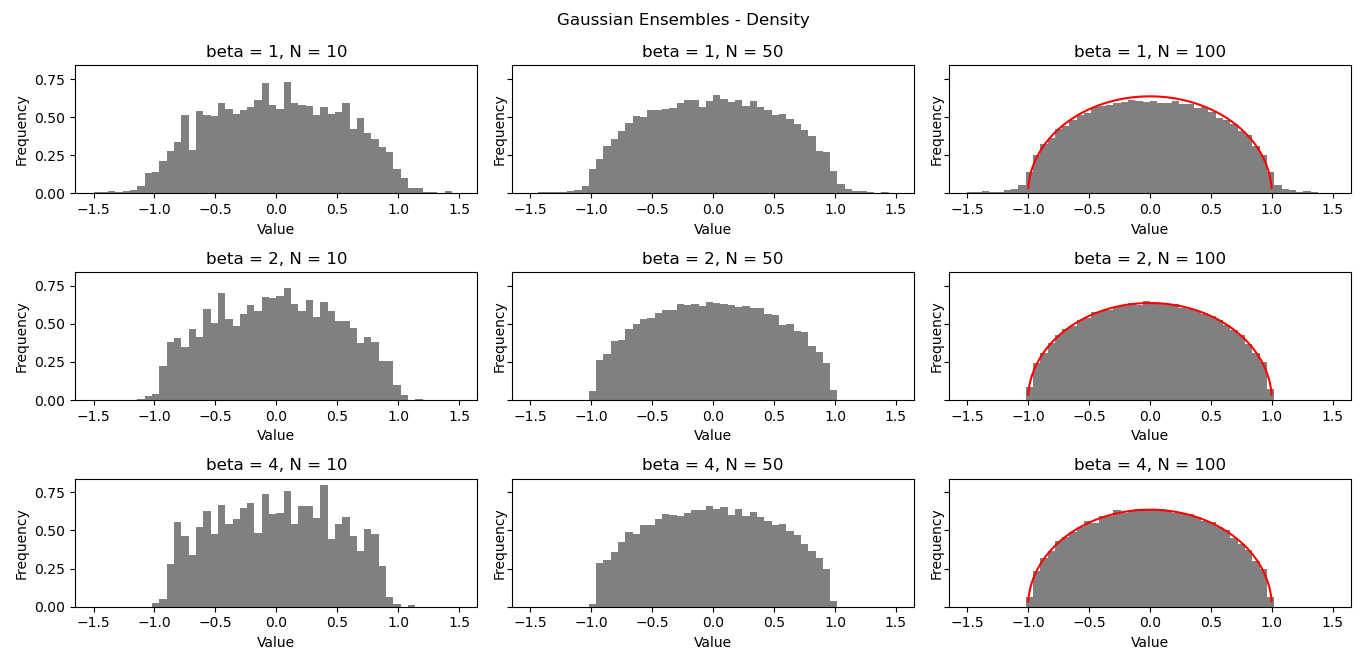
\includegraphics[scale=0.45]{Assets/validationArticleAlg}
	\caption{Validação para ensembles clássicos, utilizamos $200000$ passos registrando a cada $500$ a partir da metade dos passos. $\Delta t = 0.1$, $\gamma = 1$, $\alpha = 1.0$. Para replicar a semente foi $987991650$.}
	\label{fig: semicircle}
\end{figure}

Podemos considerar agora exemplos de potenciais que podem ser aplicados. Lembre que isso implica que nossa entradas são correlacionadas, os ensembles de matrizes para este caso não são tão diretos quanto para entradas independentes. Consideraremos para os exemplos $\beta = 2$. As explicações para os resultados gráficos são retomados na seção sobre as simulações implementadas.


\subsection{Potencial Mônico}

Considere o potencial

\[
	V(x) = \frac{t}{2\alpha} x^{2\alpha}
\]

Onde $t > 0$ é escala e $\alpha \in \Z$. A medida de equilíbrio para $\alpha = 1$ é o semi-círculo de podemos validar na figura com a distribuição em vermelho. De qualquer forma, podemos observar os resultados das simulações para este potencial e notar o comportamento esperado e a distribuição teórica em vermelho para o semicírculo \ref{fig: monic}.


\begin{figure}[ht]
	\centering
	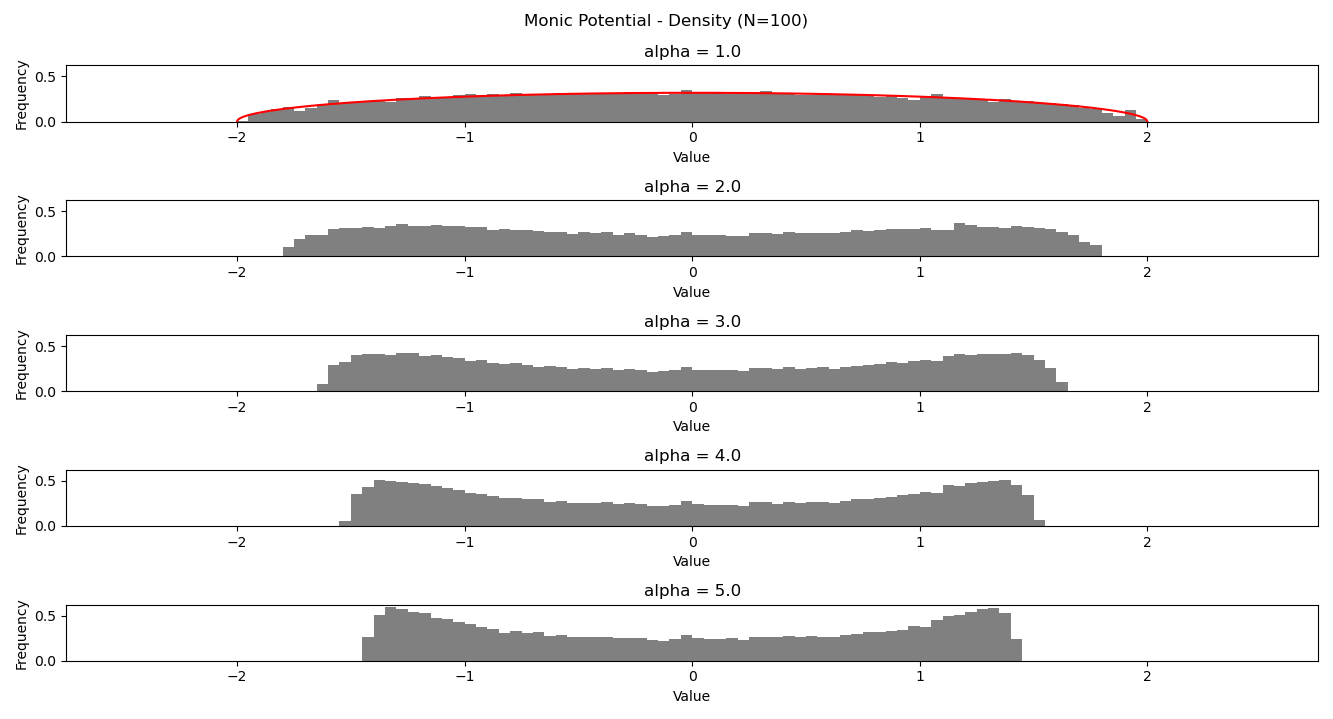
\includegraphics[scale=0.4]{Assets/validationArticleMonic}
	\caption{Validação para potencial mônico, $V(x) = \frac{t}{2 \alpha} x^{2\alpha}$. Utilizamos $1000000$ passos registrando a cada $500$ a partir da metade dos passos. $t = 1$, $\Delta t = 0.1$, $\gamma = 10$, $\alpha = 0.1$. Para replicar a semente foi $987991650$.}
	\label{fig: monic}
\end{figure}


\subsection{Potencial Quártico}

Considere o potencial

\[
	V(x) = \frac{x^4}{4} + t \frac{x^2}{2}
\]

Aqui observaremos pela primeira vez uma transição de estado. Teremos um ponto crítico em $t=-2$ onde a medida se para em dois intervalos $[-b_t, -a_t]$ e $[a_t, b_t]$. Ou seja:

\begin{itemize}
	\item t > -2
	\[
	\supp \mu_V = [-b_t, b_t], \frac{d \mu_V}{dx}(x) = \frac{1}{2\pi} (x^2 - c_t^2) \sqrt{b_t^2 - x^2} 
	\]
	
	com
	
	\[
		c_t^2 \deff\frac{1}{2} b_t^2 + t \deff \frac{1}{3} (-2t + 2 \sqrt{t^2 + 12})
	\]
	
	\item t < -2
	\[
	\supp \mu_V = [-b_t, -a_t] \cup [a_t, b_t], \frac{d \mu_V}{dx}(x) = \frac{1}{2\pi} |x| \sqrt{(x^2 - a_t^2)(b_t^2 - x^2)} 
	\]
	
	com
	
	\[
	a_t \deff \sqrt{-2-t}, b_t \deff \sqrt{2-t}
	\]
\end{itemize}

Observamos o comportamento esperado e a distribuição teórica em vermelho em \ref{fig: quartic}. 


\begin{figure}[ht]
	\centering
		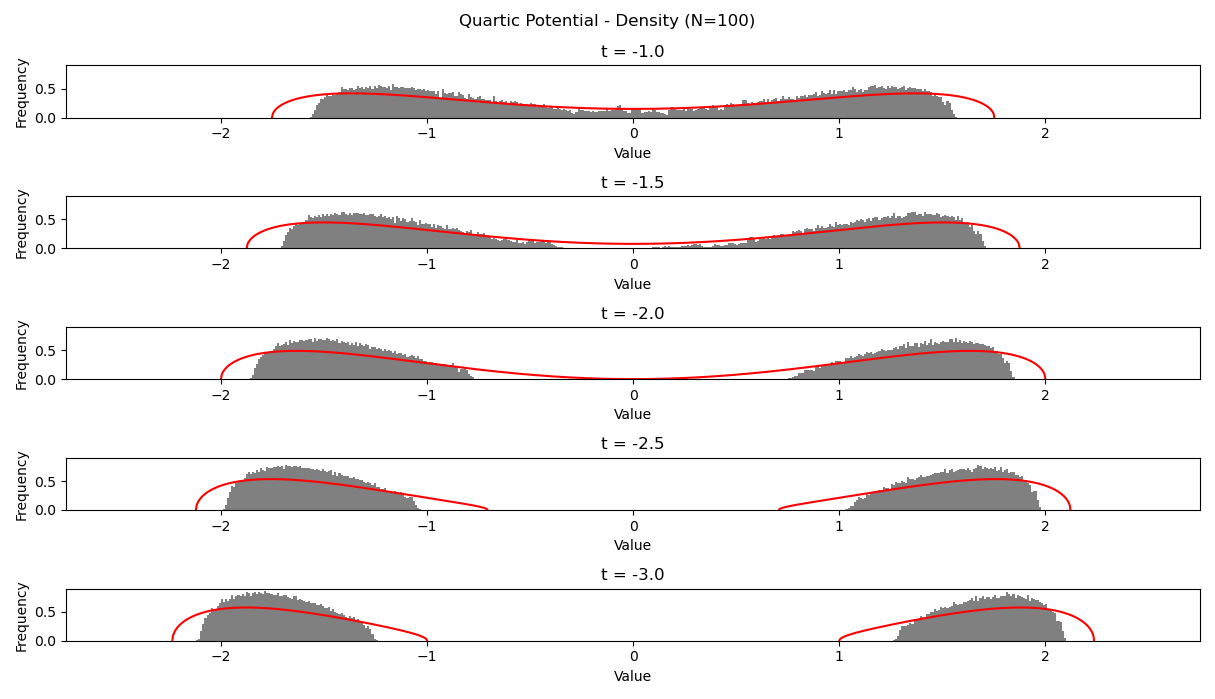
\includegraphics[scale=0.4]{Assets/validationArticleQuartic}
		\caption{Validação para potencial quártico, $V(x) = \frac{1}{4} x^4 + \frac{1}{2} x^2$. Utilizamos $1000000$ passos registrando a cada $500$ a partir da metade dos passos. $\Delta t = 0.1$, $\gamma = 10$, $\alpha = 0.1$. Para replicar a semente usada é $987991650$.}
		\label{fig: quartic}
\end{figure}


	
	\section{Simulações de Gases}
	\label{sec: simul}
	
	Recorde que um gas de coulomb é descrito pela medida explicitada em \ref{eq: coulomb}. Para alguns modelos destes gases, pode-se utilizar modelos de matrizes aleatórias com mesma medida do espectro para auxiliar na simulação de suas dinâmicas, quando estes estão disponíveis. Processos determinantais também podem ser de ajuda quando $\beta = 2$. Fora esses casos, existem ainda métodos alternativos como o \textit{Overdamped Langevin Difusion Algorithm}, \textit{Metropolis-Hastings algorithm}, \textit{Metropolis adjusted Langevin algorithm} e versões cinéticas chamadas \textit{Hybrid or Hamiltonian Monte Carlo} baseada em uma versão cinética (\textit{underdamped}) da difusão de Langevin.

Em geral amostrar a medida resulta em dificuldades. A computação de forças e de energias escala com $N^2$ pelo Hamiltoniano tratar de interações par a par. Outra dificuldade são as singularidades em $W$, que resultam em instabilidades numéricas.

\subsection{Os típicos}

A ideia explorada é que $P_N$ é medida de probabilidade invariante reversível do processo de difusão de Markov $(X_t)_{t>0}$ solução de

\[
\dd X_t = -\alpha_N \nabla H_N(X_t) \dd t + \sqrt{2\frac{\alpha_N}{\beta_N} \dd B_t}.
\]

Sob algumas condições em $\beta_N$ e $V$, podemos afirmar que

\[
X_t \xrightarrow[t \rightarrow \infty]{Law} P_N.
\]

Discretizado, tomamos o processo

\[
x_{k+1} = x_k - \nabla H_N(x_k) \alpha_N \Delta t + \sqrt{2\frac{\alpha_N}{\beta_N} \Delta t} G_k,
\]
onde $G_k$ é a família de variáveis gaussianas usuais. Uma forma de contornar o viés embutido é amenizar a dinâmica com a forma

\[
x_{k+1} = x_k - \frac{\nabla H_N(x_k) \alpha_N \Delta t}{1 + |\nabla H_N(x_k)| \alpha_N \Delta t} + \sqrt{2\frac{\alpha_N}{\beta_N} \Delta t} G_k.
\]
Ainda assim, precisamos otimizar o processo. A ideia do algoritmo de Metropolis é adicionar um processo de seleção para evitar passos irrelevantes, algo do tipo:

\begin{itemize}
	\item defina $\tilde{x}_{k+1}$ de acordo com o kernel $K(x_k, \cdot)$ gaussiano;
	
	\item defina $p_k$
	
	\[
	p_k = 1 \wedge \frac{K(\tilde{x}_{k+1},x_k) e^{\beta_N H_N(\tilde{x}_{k+1})}}{K(x_{k},\tilde{x}_{k+1}) e^{\beta_N H_N(\tilde{x}_{k})}};
	\]
	
	\item defina
	
	\[
	x_{k+1} = 
	\begin{cases}
		\tilde{x}_{k+1} & \quad \text{com probabilidade} \ \ p_k,\\
		x_k &  \quad \text{com probabilidade} \ \ 1-p_k.
	\end{cases}
	\]
	
\end{itemize}

\subsection{O Híbrido de Monte Carlo}

O algoritmo híbrido de Monte Carlo é baseado no algoritmo anterior mas adicionando uma variável de momento para melhor explorar o espaço. Defina $E = \mathbb{R}^{\dd N}$ e deixe $U_N : E \rightarrow \mathbb{R}$ ser suave para que $\ee^{-\beta_N U_N}$ seja Lebesgue integrável. Seja ainda $(X_t, Y_t)_{t>0}$ o processo de difusão em $E \times E$ solução de

\[
\begin{cases}
	\dd X_t = \alpha_N \nabla U_N (Y_t) \dd t, \\
	\dd Y_t = \alpha_N \nabla H_N(X_t) \dd t - \gamma_N \alpha_N \nabla U_N(Y_t) \dd t + \sqrt{2\frac{\gamma_N \alpha_N}{\beta_N} \dd B_t},
\end{cases}
\]
onde $(B_t)_{t>0}$ é o movimento browniano em $E$ e $\gamma_N > 0$ parâmetro representando atrito.

Quando $U_N(y) = \frac{1}{2}|y|^2$ temos $Y_t = \dd X_t/\dd t$ e teremos que $X_t$ e $Y_t$ poderão ser interpretados como posição e velocidade do sistema de $N$ pontos em $S$ no tempo $t$. Nesse caso, $U_n$ é energia cinética.

\subsubsection{O algoritmo discreto}

Descrevemos agora o algoritmo discretizado. Inicie de uma configuração $(x_0, y_0)$ e para todo $k \geq 0$ faça

\begin{enumerate}
	\item atualize as velocidades com
	
	\[
	\tilde{y}_k = \eta y_k + \sqrt{\frac{1-\eta^2}{\beta_N}} G_k, \ \eta = \ee^{-\gamma_N \alpha_N \Delta t};
	\]
	
	\item calcule os termos
	\[
	\begin{cases}
		\tilde{y}_{k+\frac{1}{2}} = \tilde{y}_k - \nabla H_N(x_k) \alpha_N \frac{\Delta t}{2}, \\
		\tilde{x}_{k+1} = x_k + \tilde{y}_{k + \frac{1}{2}} \alpha_N \Delta t, \\
		\tilde{y}_{k+1} = \tilde{y}_{k+\frac{1}{2}} - \nabla H_N(x_{k+1}) \alpha_N \frac{\Delta t}{2};
	\end{cases}
	\]
	
	\item definir $p_k$
	
	\[
	p_k = 1 \wedge \exp{\left[ -\beta_N \left(  H_N(\tilde{x}_{k+1}) + \frac{\tilde{y}^2_{k+1}}{2} - H_N(x_k) - \frac{\tilde{y}^2_k}{2} \right)\right] };
	\]
	
	\item defina
	
	\[
	(x_{k+1}, y_{k+1}) = 
	\begin{cases}
		(\tilde{x}_{k+1}, \tilde{y}_{k+1}) \ \text{com probabilidade} \ p_k, \\
		(x_k, -\tilde{y}_{k}) \ \text{com probabilidade} \ 1-p_k; \\
	\end{cases}
	\]
	
\end{enumerate}

\subsection{Discussão}

Já apresentamos ao longo do relatório alguns dos resultados das simulações nas figuras \ref{fig: semicircle} e \ref{fig: quarticmonic}. Para \ref{fig: semicircle} temos concordância do comportamento teórico assintótico (semi-círculo) e mesmo nos casos de baixo $N$, os resultados de matrizes aleatórias e da simulação concordam fortemente. Note que as simulações estão normalizadas para que o suporte seja $[-1,1]$ em \ref{fig: semicircle}.

Para o potencial mônico, podemos validar qualitativamente a forma do potencial e o efeito que causa na distribuição. O movimento da densidade para as bordas é justificado nesse sentido. Contudo, os resultados numéricos tem discrepâncias com a teoria ainda não justificadas. Um exemplo disso é o fato do suporte da densidade do resultado numérico ser visivelmente menor do que o suporte teórico.

Finalmente, para o potencial quártico, o resultado novamente é comparável a teoria em forma. Alguma ponderação pode esclarecer alguns pontos, outros ainda são injustificados. Para a quantidade de partículas consideradas, a densidade deve ser diferente da assintótica. Por exemplo, encontrar partículas em torno de $x=0$ é razoavelmente raro para os casos próximos da transição. De forma que a quantidade de passos e partículas influencia fortemente a observação de realizações na região. O suporte da densidade no resultado numérico, novamente reduzido, ainda não foi explicado.



	{\let\clearpage\relax \chapter{Plano de atividades}}\label{chp:plano}
	
	O projeto tem como base um planejamento de 12 meses, que se deram início em junho de 2023, até o momento foram realizados 5 meses de projeto.
	
	\section{Atividades Desenvolvidas}
	\label{section:atividadesdesenvolvidas}
	
	A execução do projeto foi dividida nas seguintes etapas:
	
	\begin{enumerate}
		\item \textbf{Revisão da Literatura em RMT, e estudo de teoria básica do GUE}, é necessário fazer vasta revisão de literatura no tema para que o aluno tenha domínio das ferramentas e métodos utilizados para o tratamento de matrizes aleatórias e suas implicações em mecânica estatística. Para isso, durante esse período será realizado o estudo da bibliografia adequada;
		
		\item \textbf{Estudo dos métodos de Simulação}, como mencionado, uma das aplicações importantes da teoria de matrizes aleatórias reside em sua conexão com gases de Coulomb. Em 2018 publicou-se o \cite{Chafa__2018}, artigo que é base para o estudo de métodos de simulação desses gases;
		
		\item \textbf{Implementação dos algoritmos}, implementa-se os métodos descritos no artigo e tenta-se estender seu uso em condições diferentes das utilizadas no artigo, como por exemplo em outros potenciais;
		
		\item \textbf{Redação dos Relatórios Científicos}, quando serão escritos os relatórios exigidos pelas normas da \textit{FAPESP}.
		
	\end{enumerate}
	
	\section{Cronograma}
	
	Com base nas tarefas enumeradas na Seção \ref{section:atividadesdesenvolvidas}, é mostrado na Tabela \ref{tab:cronograma1ano} o cronograma atual de desenvolvimento do projeto. Em especial, os métodos de simulação puderam ser adiantados no desenvolvimento para o mês 4, previamente previsto para o mês 5 e consequentemente as implementações também puderam ser iniciadas.


\begin{table}[ht!]
	\centering
	\begin{tabular}{|c|c|c|c|c|c|c|c|c|c|c|c|c|}
		\hline
		\multirow{2}{*}{{\bf Fases}} & \multicolumn{12}{c|}{{\bf Meses}}
		\\ \cline{2-13}
		& 1 & 2 & 3 & 4 & 5 & 6 & 7 & 8 & 9 & 10 & 11 & 12
		\\ \hline
		{\bf 1. Revisão Literatura RMT} & \checkmark & \checkmark & \checkmark & \checkmark & \checkmark & & & & & & &
		\\ \hline
		{\bf 2. Métodos de Simulação} &  &  &  & \checkmark & \checkmark & x & x & x & & & &
		\\ \hline
		{\bf 3. Implementação algoritmos} & & & & & \checkmark & x & x & x & x & x & x &
		\\ \hline
		{\bf 4. Redação Relatórios} & & & & \checkmark & \checkmark & & & & & & x & x 
		\\ \hline
	\end{tabular}
	\caption{Cronograma das atividades.}
	\label{tab:cronograma1ano}
\end{table}
	
	{\let\clearpage\relax \chapter{Participação em eventos científicos}}\label{chp:particEvento}
	
		O bolsista apresentou em dois eventos no período em que se refere o presente relatório. O Colóquio Brasileiro de Matemática (CBM) e a Semana Integrada da Física de São Carlos (SIFSC). Apenas para o primeiro, realizado no Rio de Janeiro, foi necessário o uso da reserva técnica. Por isso, segue o pôster apresentado na página que se segue. O trabalho é complementar aos estudos assintóticos e de probabilidade realizados nos meses cobertos por este relatório.

\hspace{1cm}

\begin{tabular}{|c|c|c|c|c|c|}
	\hline
	Evento &  Sede & Data & Modalidade & Apresentação & Reserva Técnica \\
	\hline
	CBM & IMPA & 24-28/07/23 & Presencial & Pôster - Oral & Sim \\
	\hline
	SIFSC & IFSC-USP & 21-25/08/23 & Presencial & Pôster - Oral & Não \\
	\hline
\end{tabular}

\hspace{1cm}

O trabalho apresentado no CBM foi apresentado oralmente por meio de pôsteres no evento científico Colóquio Brasileiro de Matemática ocorrido de 24-28 de Julho no IMPA, Rio de Janeiro. Foram utilizadas duas diárias da reserva para a participação do colóquio.


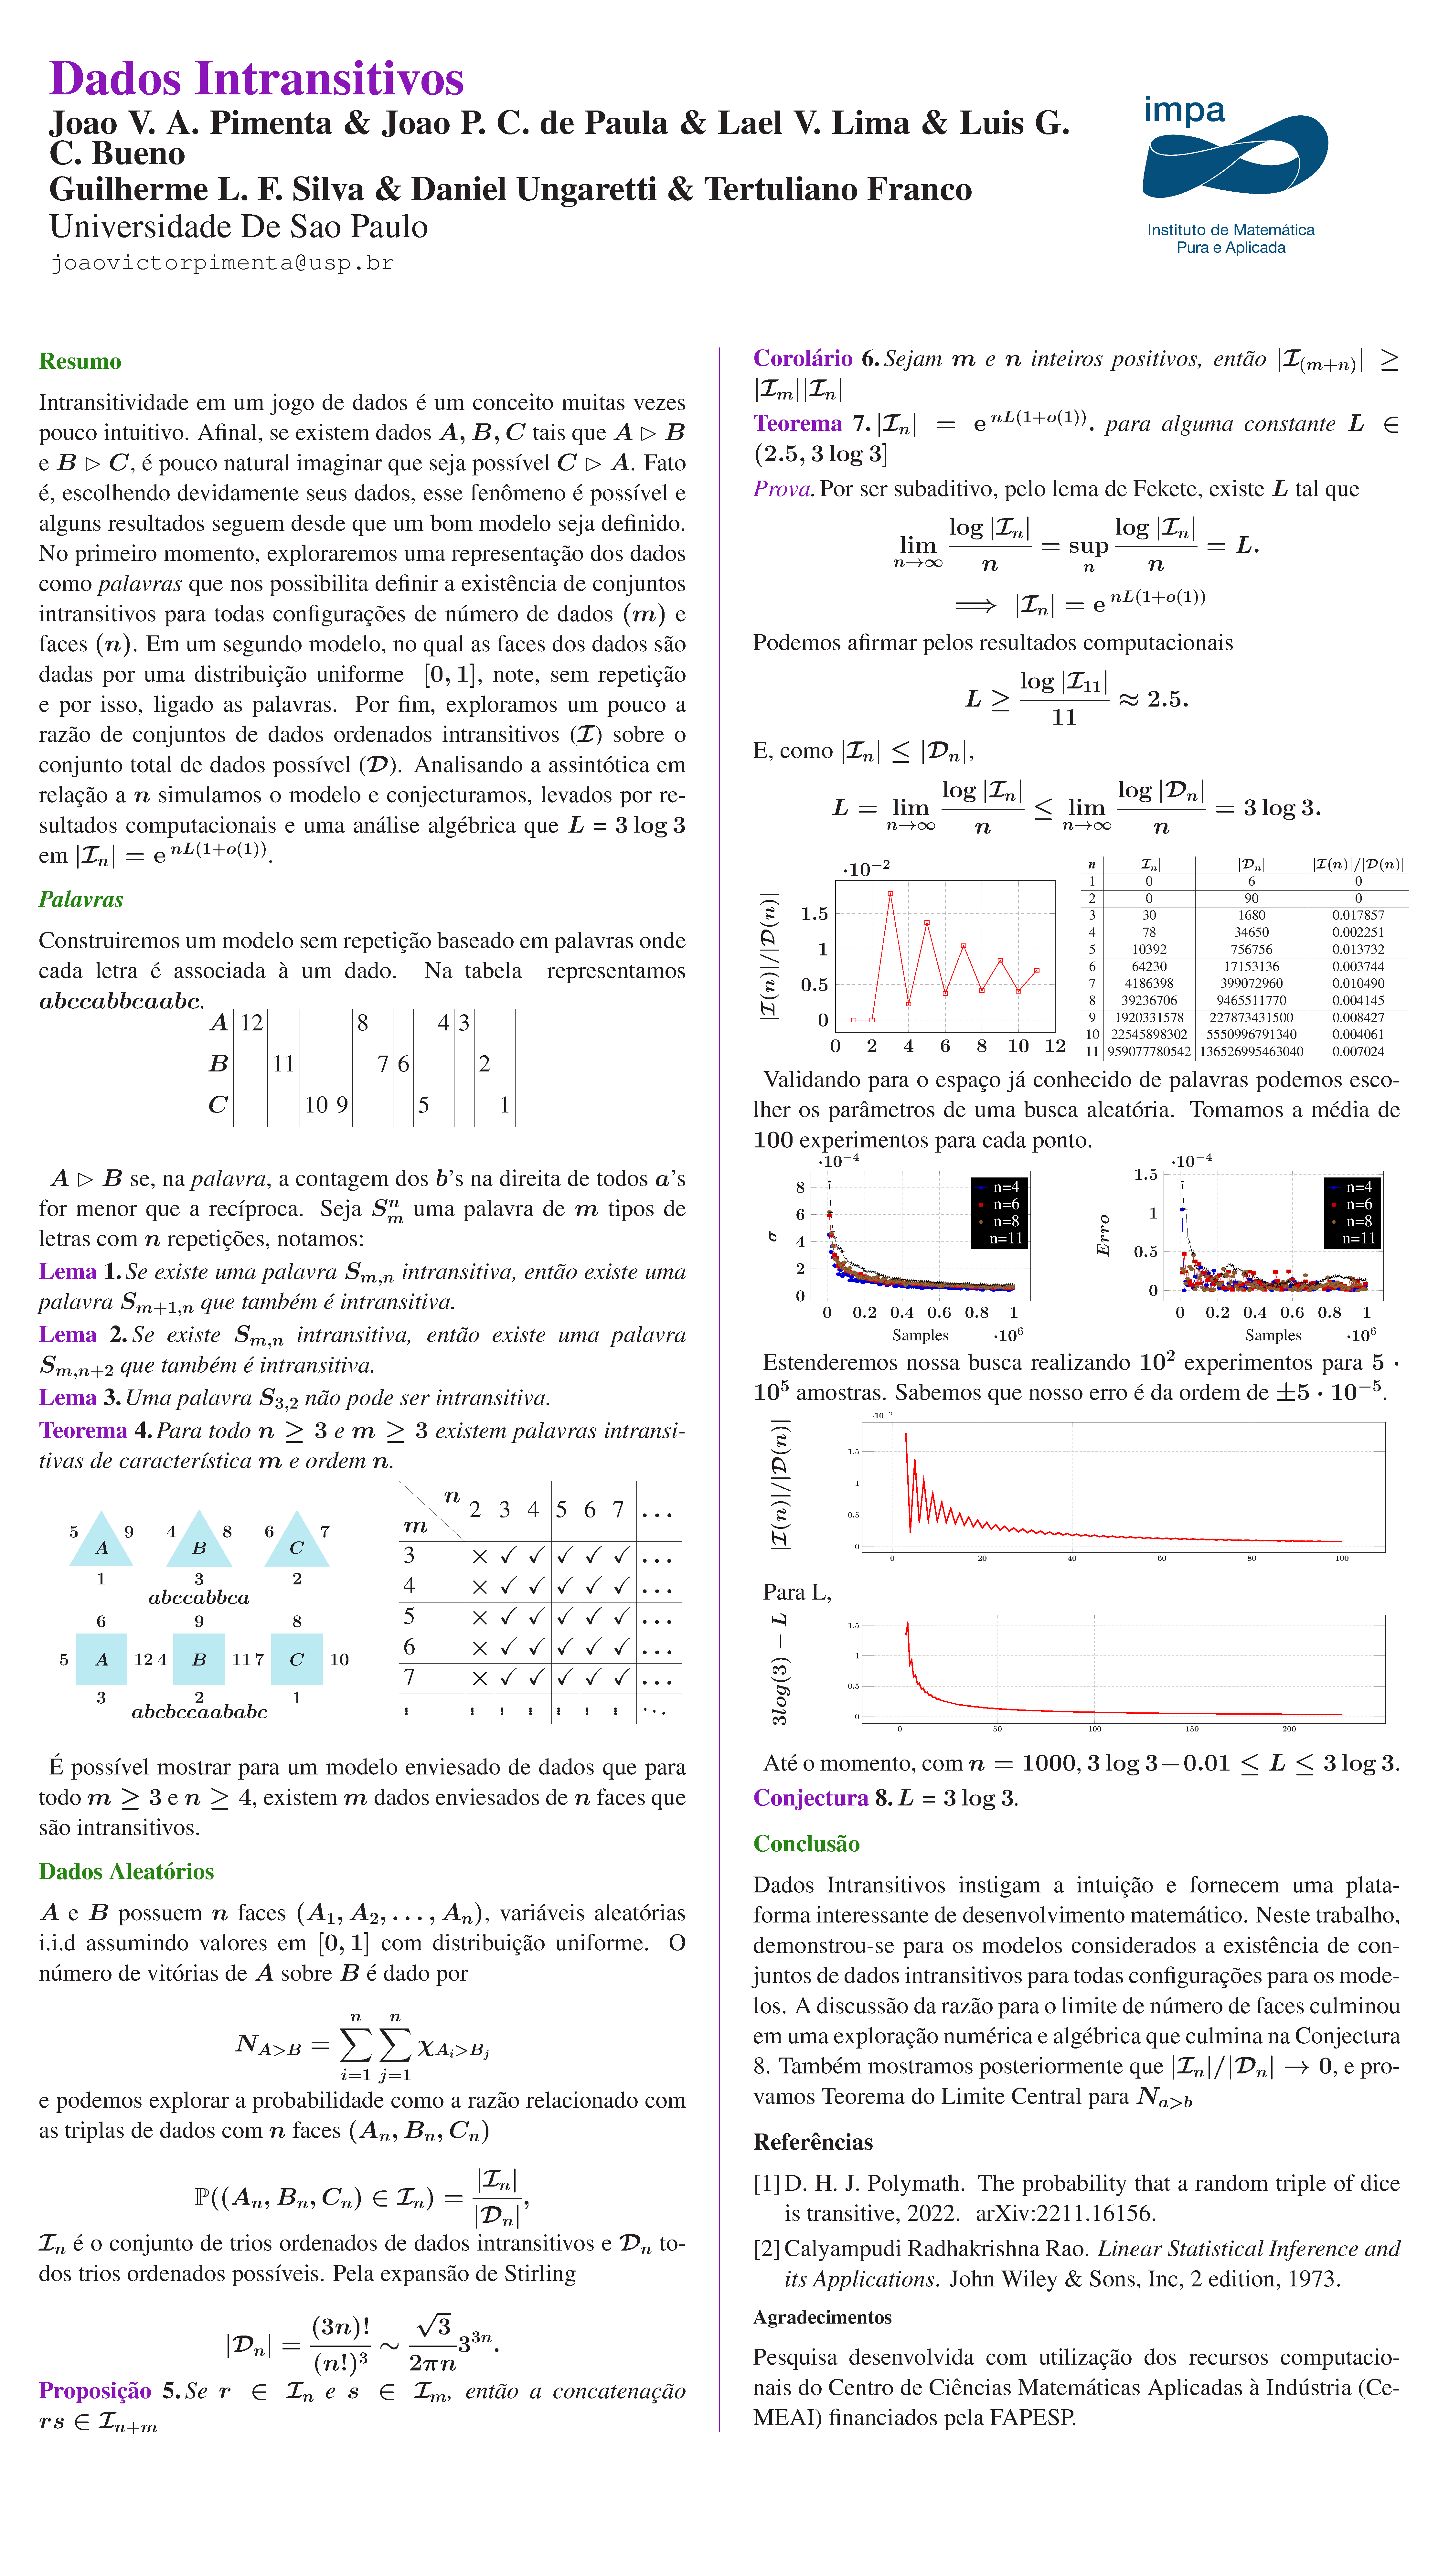
\includepdf[pages={1}]{Assets/posterwhite.pdf}
	
	{\let\clearpage\relax \chapter{Outros trabalhos Preparados ou Submetidos}}\label{chp:trabalhos}
	
	Durante o período da bolsa foi também finalizado o trabalho intitulado 'A Central Limit Theorem for intransitive dice' co-autorado por mim. O arquivo se encontra disponível na plataforma Arxiv em \href{https://doi.org/10.48550/arXiv.2310.17083}{A Central Theorem for intransitive dice}\footnote{https://doi.org/10.48550/arXiv.2310.17083}.
	
	%%-----
	%% Referências bibliográficas
	%%-----
	\addcontentsline{toc}{chapter}{\bibname}
	\bibliographystyle{abntex2-num}
	\bibliography{bibliografia}
	
	%%-----
	%% Fim do documento
	%%-----
	
	%\appendix
	%\chapter{Implementação Algoritmo}
	
	%\inputminted[
	%frame=lines,
	%framesep=2mm,
	%baselinestretch=1.2,
	%bgcolor=white,
	%fontsize=\footnotesize,
	%linenos
	%]{FORTRAN}{Assets/HKMC.f}
	
\end{document}